\chapter{Segmentaciones con otros algoritmos}

\begin{table}
\centering
\resizebox*{12.75cm}{!}{
\begin{tabular}{c|c|c|c} 
\bb {U. global} & \bb {U. de Otsu} &{\bb \em K-means}&\bb {Max. entropía Renyi}\\\hline\hline
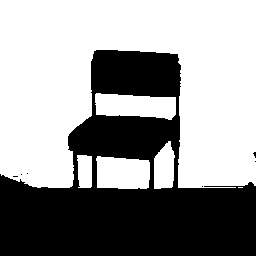
\includegraphics[width=0.2\textwidth]{img/otraseg/global-chair.jpg} &
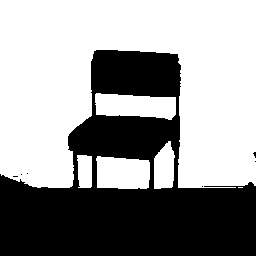
\includegraphics[width=0.2\textwidth]{img/otraseg/otsu-chair.jpg} &
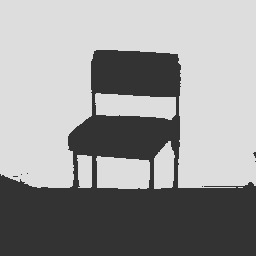
\includegraphics[width=0.2\textwidth]{img/otraseg/kmeans-chair.jpg} &
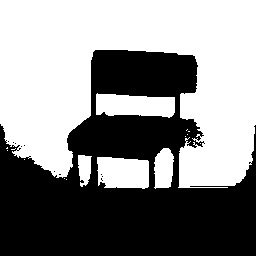
\includegraphics[width=0.2\textwidth]{img/otraseg/renyi-chair.jpg} \\
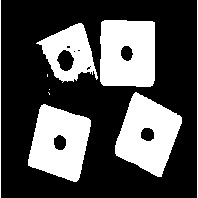
\includegraphics[width=0.2\textwidth]{img/otraseg/global-block.jpg} &
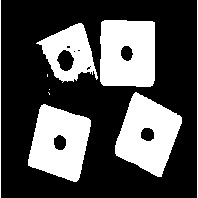
\includegraphics[width=0.2\textwidth]{img/otraseg/otsu-block.jpg} &
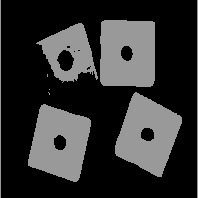
\includegraphics[width=0.2\textwidth]{img/otraseg/kmeans-block.jpg} &
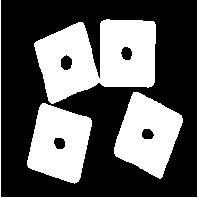
\includegraphics[width=0.2\textwidth]{img/otraseg/renyi-block.jpg} \\
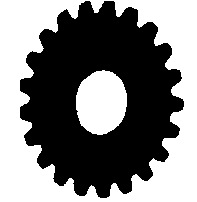
\includegraphics[width=0.2\textwidth]{img/otraseg/global-02.jpg} &
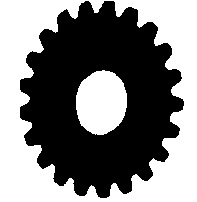
\includegraphics[width=0.2\textwidth]{img/otraseg/otsu-02.jpg} &
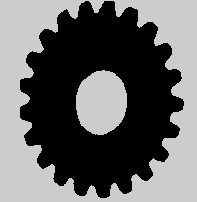
\includegraphics[width=0.2\textwidth]{img/otraseg/kmeans-02.jpg} &
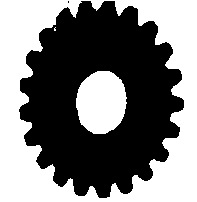
\includegraphics[width=0.2\textwidth]{img/otraseg/renyi-02.jpg} \\
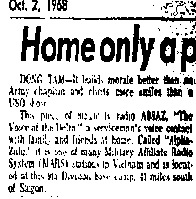
\includegraphics[width=0.2\textwidth]{img/otraseg/global-09.jpg} &
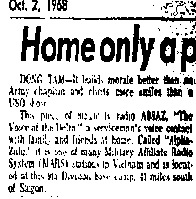
\includegraphics[width=0.2\textwidth]{img/otraseg/otsu-09.jpg} &
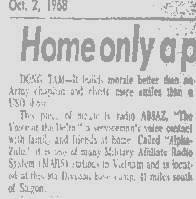
\includegraphics[width=0.2\textwidth]{img/otraseg/kmeans-09.jpg} &
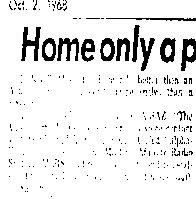
\includegraphics[width=0.2\textwidth]{img/otraseg/renyi-09.jpg} \\
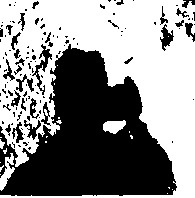
\includegraphics[width=0.2\textwidth]{img/otraseg/global-07.jpg} &
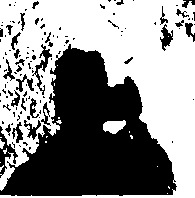
\includegraphics[width=0.2\textwidth]{img/otraseg/otsu-07.jpg} &
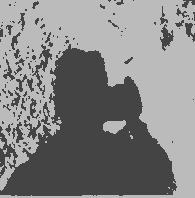
\includegraphics[width=0.2\textwidth]{img/otraseg/kmeans-07.jpg} &
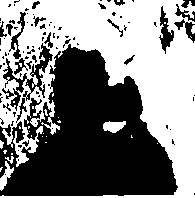
\includegraphics[width=0.2\textwidth]{img/otraseg/renyi-07.jpg} \\\hline
\end{tabular}}
\caption{Segmentaciones para las imágenes con los algoritmos de otros autores.\label{tab:otrassegmentaciones}}
\end{table}

Los cuadros que se presentan en este apéndice pretenden ayudar al lector a interpretar los resultados presentados a lo largo de la memoria, conociendo el resultado de otros métodos de segmentación. Con ayuda de estos se puede hacer un análisis visual de los resultados enaminado a facilitar las conclusiones a buscar.\par


\begin{table}
\centering
\resizebox*{12.75cm}{!}{
\begin{tabular}{c|c|c|c} 
\bb {U. global} & \bb {U. de Otsu} &{\bb \em K-means}&\bb {Max. entropía Renyi}\\\hline\hline
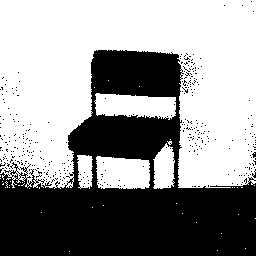
\includegraphics[width=0.2\textwidth]{img/otraseg/global-chairga.jpg} &
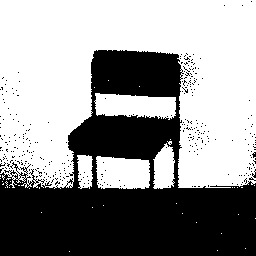
\includegraphics[width=0.2\textwidth]{img/otraseg/otsu-chairga.jpg} &
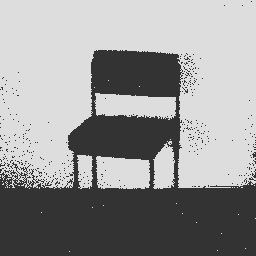
\includegraphics[width=0.2\textwidth]{img/otraseg/kmeans-chairga.jpg} &
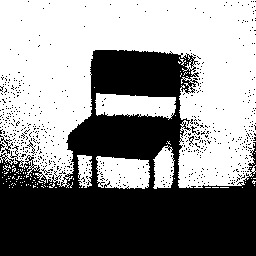
\includegraphics[width=0.2\textwidth]{img/otraseg/renyi-chairga.jpg} \\\hline
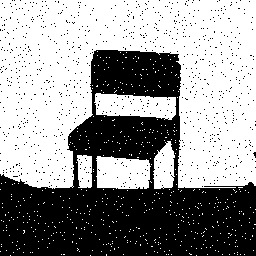
\includegraphics[width=0.2\textwidth]{img/otraseg/global-chairsp005.jpg} &
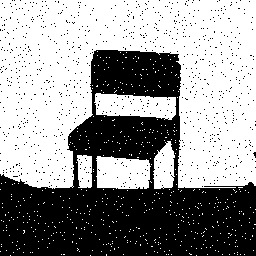
\includegraphics[width=0.2\textwidth]{img/otraseg/otsu-chairsp005.jpg} &
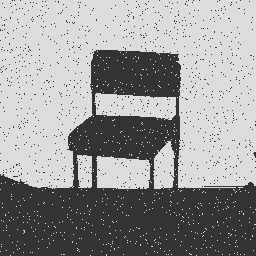
\includegraphics[width=0.2\textwidth]{img/otraseg/kmeans-chairsp005.jpg} &
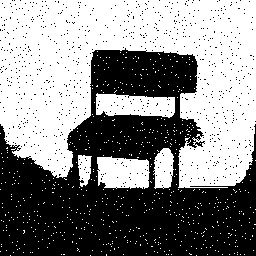
\includegraphics[width=0.2\textwidth]{img/otraseg/renyi-chairsp005.jpg} \\\hline
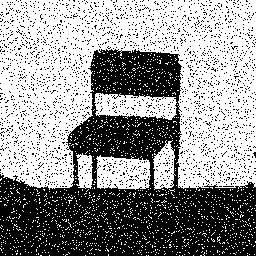
\includegraphics[width=0.2\textwidth]{img/otraseg/global-chairsp020.jpg} &
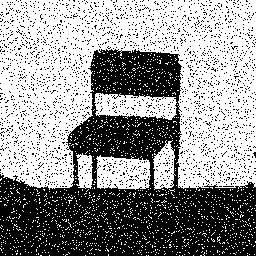
\includegraphics[width=0.2\textwidth]{img/otraseg/otsu-chairsp020.jpg} &
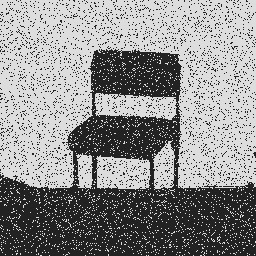
\includegraphics[width=0.2\textwidth]{img/otraseg/kmeans-chairsp020.jpg} &
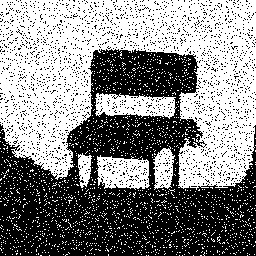
\includegraphics[width=0.2\textwidth]{img/otraseg/renyi-chairsp020.jpg} \\\hline
\end{tabular}}
\caption{Segmentaciones para las imágenes con ruido a través de los algoritmos de otros autores.\label{tab:otrassegmentaciones}}
\end{table}